\documentclass[11pt]{article}
\usepackage[english]{babel}
\usepackage{a4wide}
\usepackage[utf8]{inputenc}
\usepackage{natbib}
\usepackage{enumitem}
\usepackage{graphicx}
\setlist{itemsep=0.1em}
\usepackage{hyperref}
\usepackage{xcolor}
\definecolor{dark-red}{rgb}{0.4,0.15,0.15}
\definecolor{dark-blue}{rgb}{0.15,0.15,0.4}
\definecolor{medium-blue}{rgb}{0,0,0.5}
\hypersetup{
    colorlinks, linkcolor={black},
    citecolor={dark-blue}, urlcolor={medium-blue}
}
\setcounter{tocdepth}{2}
\bibliographystyle{agsm}
\begin{document}

\title{Mobile Application Development \\ Minor Assignment A \\ Indoor Tracking}
\author{Jonathan Mackenzie\\ 2084684}
\maketitle
\section{Functionality}
My indoor tracking application has the following functionalities: 
\begin{enumerate}
\item Tracking the location of the user through dead reckoning, utilising the orientation sensor and accelerometer data. The user's orientation is displayed with green and blue lines (blue is the orientation sensor, and green is the derived sensor value).
\item When a step is detected, a footstep sound is played. Upon resetting the user's position, another sound is played.
\item Resetting of the user's location by tapping on the map. A long tap will set the user's location to where the tap occurred.
\item Setting of the user's height and sex through a preferences activity. This activity also allows the configuration of the window size, step threshold and step timeout under advanced options.
\item A help activity that briefly explains how to use the app.
\item A graph activity that shows the current accelerometer data and the steps detected under mean and median filtering. The thresholds and window size can also be configured here and the graph paused. The steps appear as dots on the map with the last mean or median value depending on the options set at the bottom of the view.  

\end{enumerate}
\section{Investigation}
I didn't really do any formal research for this application, most of my investigation was centred around stackoverflow discussions of specific issues I had when developing for android and the android documentation. I also discussed with another student how the sensor data could be interpreted and I after implementing mean and median filtering I settled on mean filtering and the thresholds used for step detection after significant testing.

The median and mean filtering takes the last \verb+window_size+ elements from the accelerometer data and calculates the median and mean respectively. If this value exceeds  \verb+stepThreshold+ then a step has occurred. It must also occur on a timeout since the previous step in order to prevent a single peak in the data being detected as multiple steps. Originally I also checked if the gradient of the graph was near 0, but this wasn't necessary. My implementation is based off the description on the wikipedia article for median filtering (\url{http://en.wikipedia.org/wiki/Median_filter}).

The low pass filter removes the gravity factor from the sensor data and smooths the graph to some degree by making the current value a weighted average. I got the idea for this from a stackoverflow answer (\url{http://stackoverflow.com/a/15380749/150851}).

My programmer's log and source code for this assignment is available here: \url{https://github.com/JonnoFTW/IndoorTracking/commits/master}

\section{Results}

I have come to the conclusion that dead reckoning is not a useful means of tracking location within a building because magnetic fields from things like electrical cupboards, metal railings, computers, metal door frames tend to affect the orientation of the device. When using the deprecated orientation sensor, the rotation of the device was indicated with a blue line. When walking, this line indicated that the sensor was being affected by magnetic fields. The app also shows a green line (this is indicates the orientation from the derived sensor), this was also pulled, but not as much as the orientation sensor.

The results of my test are indicated in image [\ref{fig:test_path}], I walked from the door to 307, north past the railings (which pulled the path towards them), right past the elevator, down the office corridor (and past an electrical cupboard which pulled the path east), into Paul Calder's office, back to the corridor and down to Brett Wilkinson's office. The path then rerturns directly to 307 and to a lab computer at the back.

\begin{figure}[p]
\centering
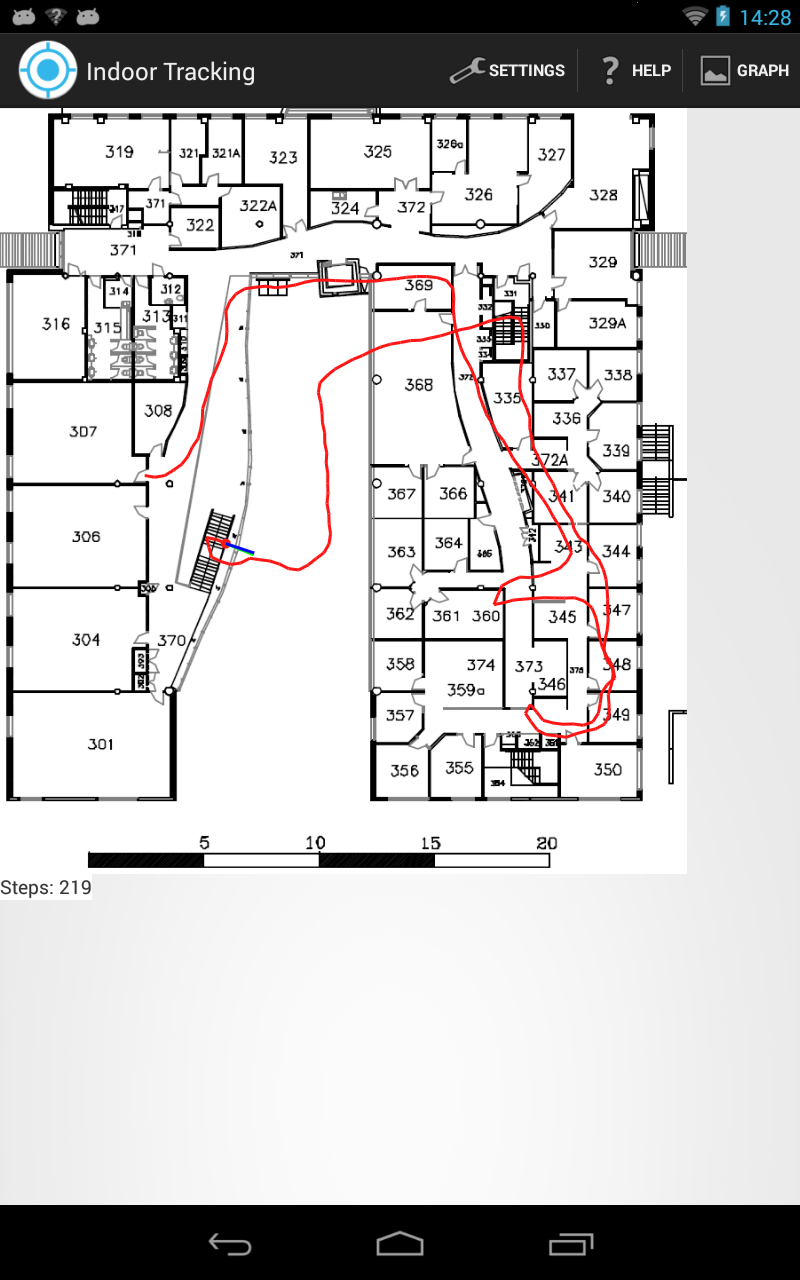
\includegraphics[width=0.8\textwidth]{screenshot.png}
\caption{My test path}
\label{fig:test_path}
\end{figure}
\end{document}